\chapter{Introducción y motivación}
\title{Introducción y motivación}
\title{Bandas de música y su problema}
\section{Bandas de música y su problema}

Los directores de orquesta tienen como función la de guiar a los miembros de dicho
grupo en la interpretación de las distintas composiciones (ya sea para realizar correcciones
durante los ensayos, elegir qué obras integrar en el repertorio, aportar un punto de expresividad
en la entonación...).\\

Sin embargo, durante un concierto hay un cometido elemental: otorgar unidad entre los instrumentos
(señalar para que todos los músicos sigan el mismo ritmo -y mantener dicha velocidad durante toda la
obra-, por ejemplo).\\

A esto hay que añadirle la dificultad que se presenta cuando bandas de música, profesionales o no,
realizan algún tipo de desfile o pasacalles donde el director no está visible a todos los músicos y,
por tanto, la tarea descrita anteriormente se hace muy difícil (o imposible) de llevar a cabo.\\

Este trabajo se centrará en tratar de remediar esta problemática.


\title{Soluciones actuales}
\section{Soluciones actuales}

Como principal solución a este problema se generaliza la utilización metrónomos durante los ensayos y,
al actuar en la calle, tratar de conseguir el mismo resultado.\\

Con el despegue de los teléfonos inteligentes, han aparecido múltiples aplicaciones que hacen las veces
de metrónomo (incluso, algunas son capaces de calcular el “tempo” -término que se verá con más detenimiento
después- a partir de las pulsaciones que haga el usuario sobre un botón -esas pulsaciones se deberán hacer
al ritmo que vaya la música-).\\

Por otro lado, los compositores han introducido algún tipo de percusión a sus obras con la finalidad de favorecer
el acompasamiento entre todos los instrumentos (además de añadir un instrumento que ayude a enriquecerlas). Si
unimos estos dos hechos, instalando una aplicación de esta naturaleza en un teléfono móvil y éste a su vez en un
soporte para un instrumento de percusión, podríamos mantener la velocidad de interpretación durante la actuación con
un coste relativamente bajo (aunque se mantiene la velocidad en el punto de referencia -que al no ser un computador,
estará sujeto a errores-, no se consigue solucionar totalmente la descoordinación entre los músicos).\\


\title{Conceptos previos necesarios}
\section{Conceptos previos necesarios}
Para poder entender algunos conceptos que se usarán a lo largo de este trabajo y hablar con propiedad en cuanto a
algunos conceptos, es necesario tener unos conocimientos musicales mínimos. Se procede a definir algunos conceptos:

\begin{itemize}
\item Pentagrama: es el conjunto formado por cinco líneas paralelas entre sí y los cuatro espacios que quedan entre ellas. Aunque también puede haber líneas adicionales por encima y por debajo del pentagrama, principalmente se usan estas cinco líneas y espacios para escribir los símbolos musicales (ya sean notas, silencios...).
  \begin{figure}[htb]
  \centering
  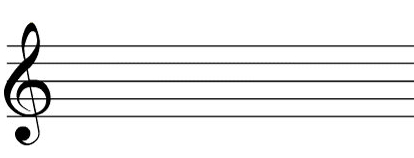
\includegraphics[width=0.8\textwidth]{./imagenes/pentagrama}
  \caption{Representación gráfica de un pentagrama} \label{fig:pentagrama}
  \end{figure}
\item Pulso: es el latido constante y regular de la música, siendo la unidad temporal básica y, en comparación con esta unidad de tiempo, se mide la duración de las notas y silencios.
\item “Tempo”: es la velocidad del pulso. Para indicar un tempo se utiliza como unidad los “bpm” (“Beats Per Minute”, es decir, los “Pulsos Por Minuto”). Así, si el tempo de una obra es de 60 bpm, tendremos que se producirá un pulso por segundo (1 bps) o lo que es lo mismo, cada un segundo, tendremos un pulso.
\item Ritmo: es la combinación de sonidos y silencios de diferente duración.
\item Compás: facilita la lectura de la música. En un pentagrama, los compases quedan divididos por líneas divisorias. Tomaremos que todos los compases son cuaternarios de subdivisión binaria (la mayoría de las obras para banda de música se encuentran compuestas para este tipo de compases o binarios -encajables en los anteriores- y así podremos simplificar el problema para su estudio aunque, como veremos durante la fase de implementación, esto es solo importante para entender mejor el diseño), es decir, un compás está dividido en cuatro notas negras (cada una será de un pulso de duración).
\end{itemize}

Cabe ahora preguntarse entre qué valores se mueve el tempo, es decir, cual es el rango
del tempo. Existen desde composiciones con menos de 20 pulsaciones por minuto hasta
otras que sobrepasan los 240. Sin embargo, no se puede perder de vista
el público al que se orienta este sistema y, cuyas composiciones, se mueven entre las 70 y 120 pulsaciones
por minuto (dependerá de la composición).\\

Si el lector tiene dudas sobre estos conceptos o desea ampliarlos, puede consultar
la bibliografía \cite{teorMusica} \cite{lenguajeMusical}.\\


\title{Producto a desarrollar}
\section{Producto a desarrollar}

Teniendo en cuenta todo lo dicho en las anteriores páginas, es el momento de manifestar
qué dispositivo es el que se desea desarrollar en este trabajo: un sistema que marque el
pulso (que no el ritmo, al poder ser éste irregular mientras que el pulso es constante)
en función del “tempo” que indique el director de la agrupación. Además, el sistema deberá
ser discreto ya que se busca que las bandas lo utilicen principalmente en la calle.\\

Esta necesidad por parte de las bandas de música ha sido detectada por algunos fabricantes,
como Peterson, que puso a la venta un producto llamado “Body Beat”. Dispone de un amplio
abanico de funciones, pero su tamaño y su elevado coste hacen inviable la implantación del
sistema en una banda de música (hay que tener en cuenta que el número de componentes en una
banda es variable pero ronda entre los 50 y 100 músicos -algunas de ellas sobrepasan este número,
como la ``Banda de Cornetas y Tambores Nuestra Señora de la Victoria" conocida como ``Las Cigarreras"
de Sevilla \cite{cigarreras} que, en las fechas en las que se escribe este trabajo, ronda los 140 componentes-.
Por otro lado, las dimensiones, de unos 10.8 cm x 7.6 cm x 2.54 cm puede que sean demasiado grandes).
Como último punto a tener en cuenta, muchos son los usuarios que, a través de diversas páginas en Internet,
se lamentan de la corta duración de la batería (teniendo en cuenta que hay actuaciones que pueden llegar a
durar entre 8 y 10 horas, esto es un problema importante).\\


\begin{figure}[htb]
\centering
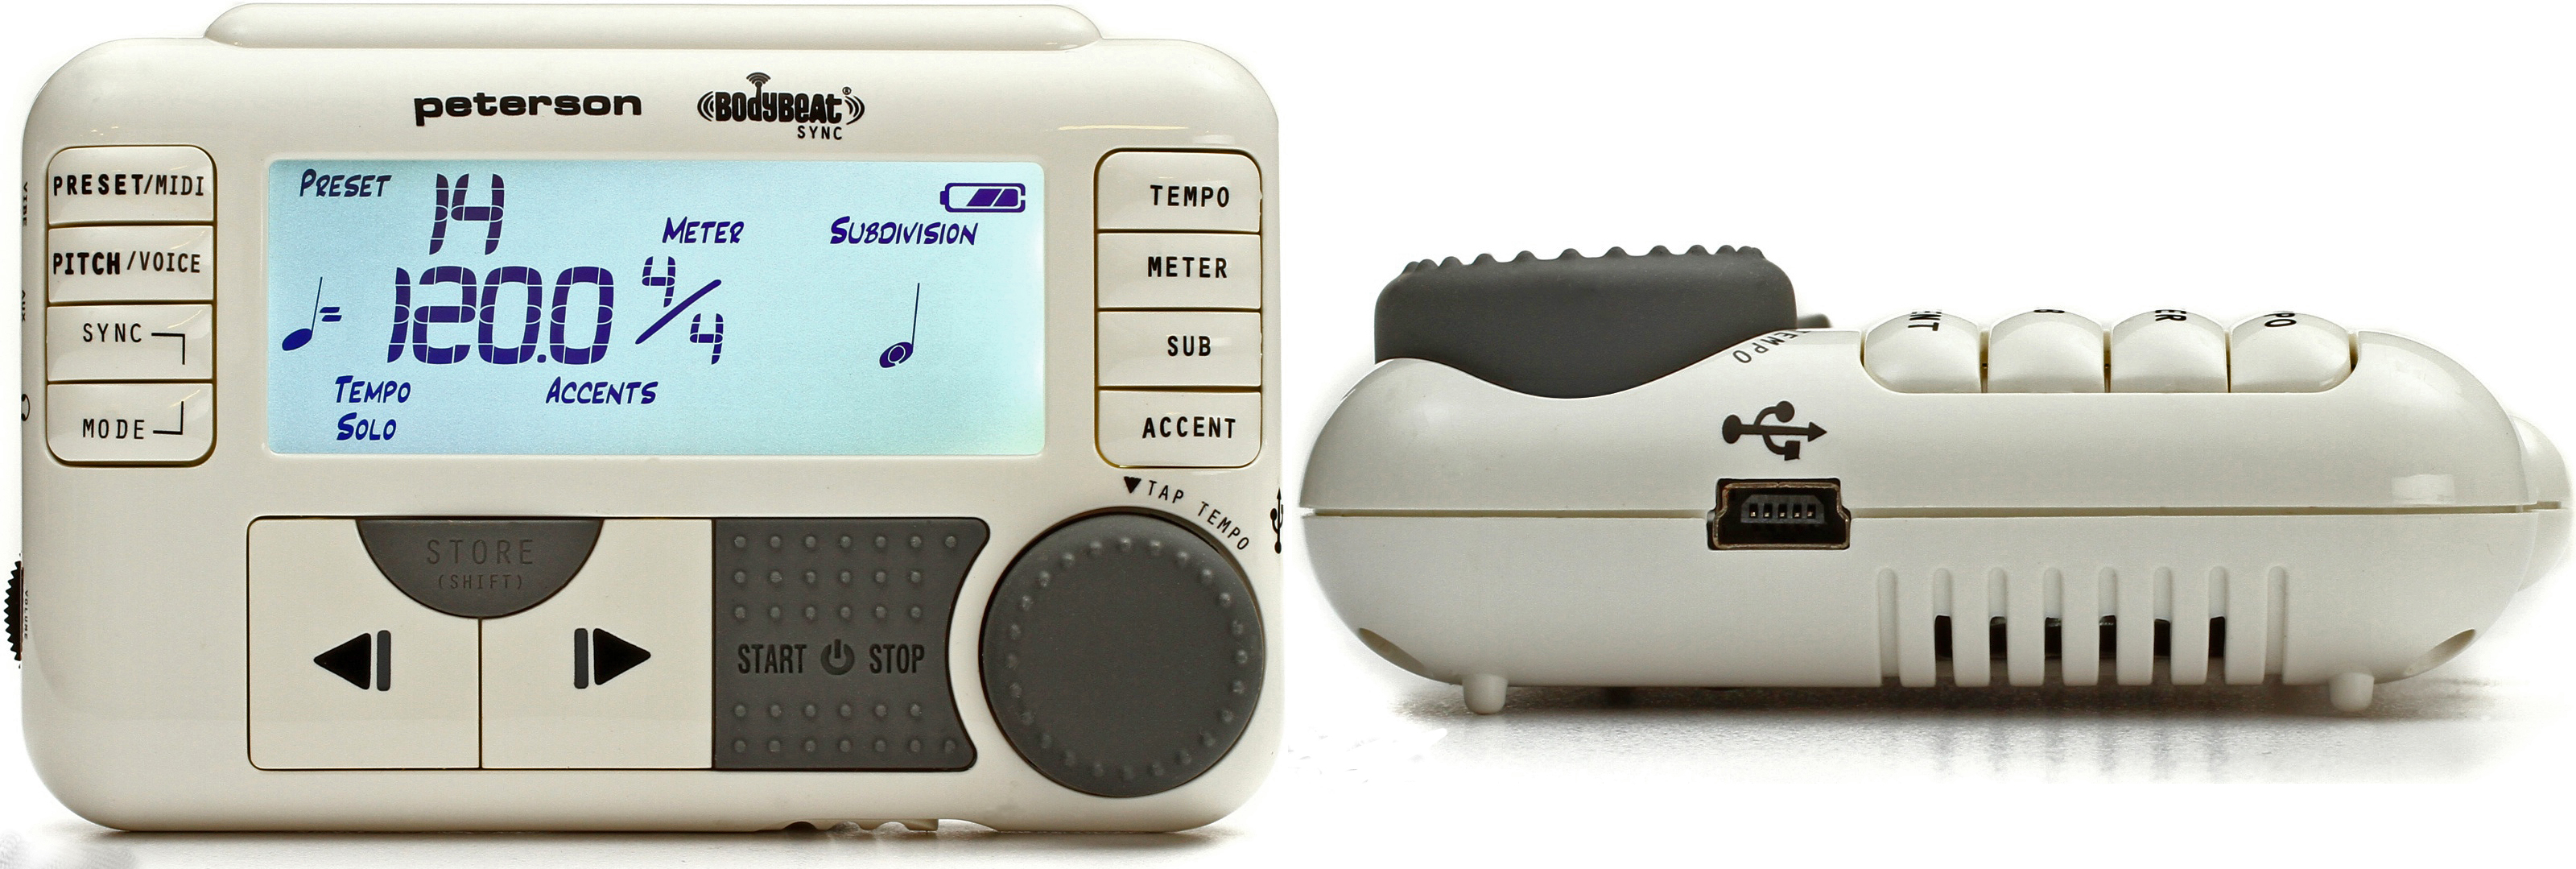
\includegraphics[width=0.6\textwidth]{./imagenes/bodybeat}
\caption{``Body Beat" de la marca Peterson. Imagen extraída de
\scriptsize{http://www.petersontuners.com} \label{fig:bodybeat}}
\end{figure}

Un dispositivo más barato con un número menor de funciones pero que permita la sincronización de todos
los dispositivos y mantener el tempo durante toda la interpretación, atraería más usuarios. Si además
se procura que la construcción se haga utilizando software y hardware libre, podría crearse una comunidad
de desarrolladores en torno al producto, consiguiendo mejorar la calidad del dispositivo y aumentar la funcionalidad
de este.\\
